\section{Transistor come emitter follower}

Per assemblare i seguenti circuiti, non avendo più bisogno della decade di resistenze e del LED, abbiamo deciso di smontare il circuito precedente e ricominciare \emph{ex novo}.

\begin{wrapfigure}[6]{r}[0pt]{36mm}
	\caption{cc3}
	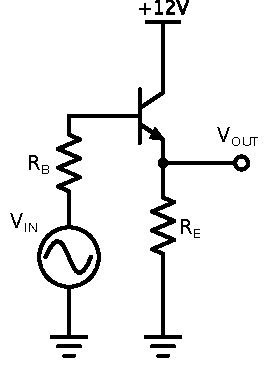
\includegraphics[height=45mm]{cc3.pdf}
	\label{fig:cc3}
\end{wrapfigure}

\subsection{emitter follower}
Il nuovo circuito, mostrato in Fig. \ref{fig:cc3}, è stato alimentato tramite il generatore di forme d'onda con un'onda sinusoidale ad una tensione picco-picco $V_{pp} = \SI{10}{\volt}$. Per osservare il segnale in uscita è stato collegato l'oscilloscopio all'emettitore del transistor.

\begin{figure}[h]
\center
	\caption{Nel grafico a sinistra sono rappresentati i segnali in input e in output al circuito del emitter follower semplice, mentre a destra sono rappresentati i segnali dell'emitter follower polarizzato. Entrambi i segnali sono stati ricavati con una frequenza di $V_{in}$ di \SI{20}{\kilo\hertz}.}
	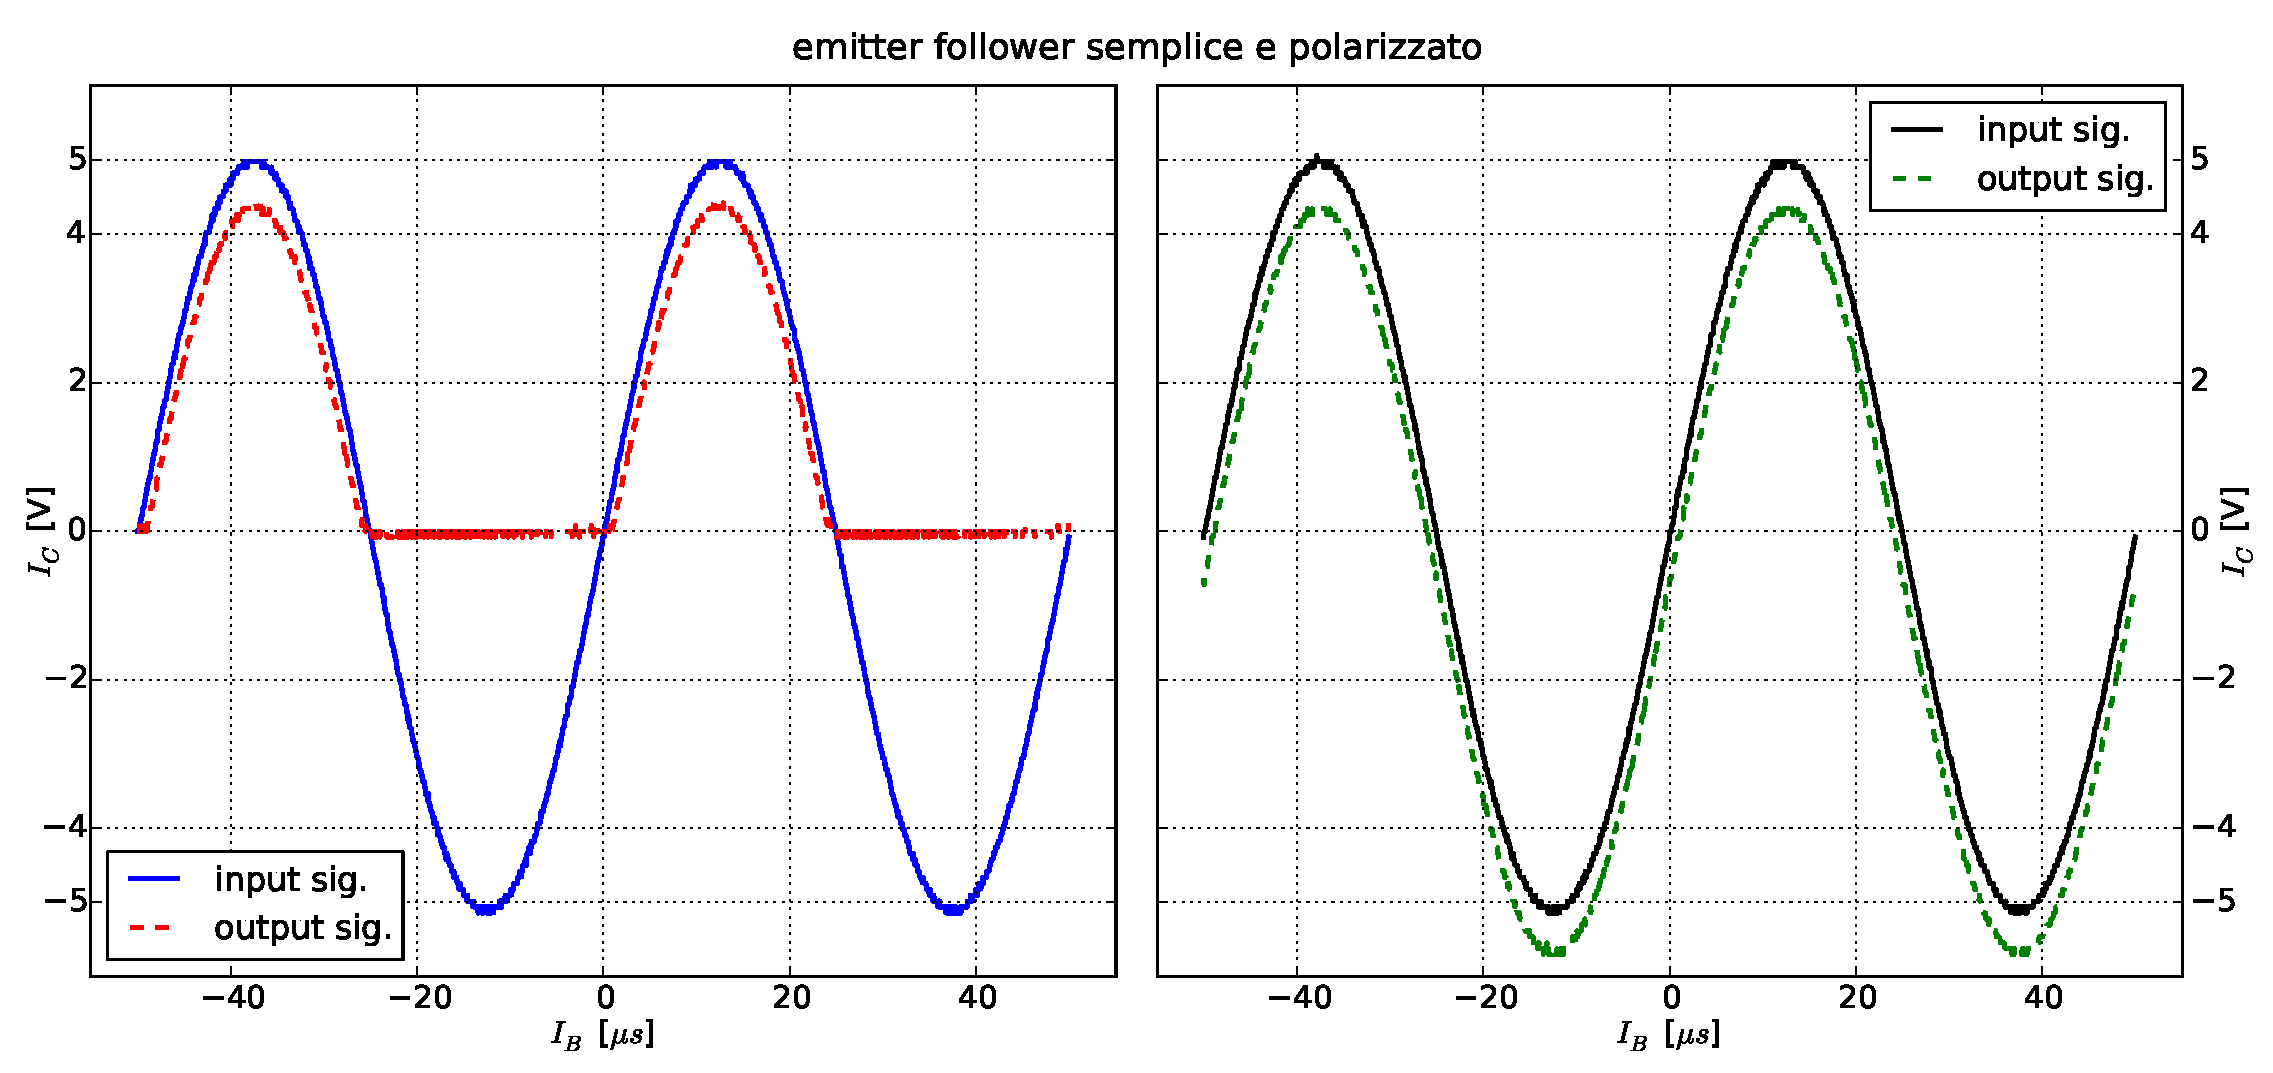
\includegraphics[width=0.85\textwidth]{cc3+cc4.pdf}
	\label{fig:cc3+cc4}
\end{figure}

\begin{wrapfigure}[6]{r}[0pt]{36mm}
	\caption{cc4}
	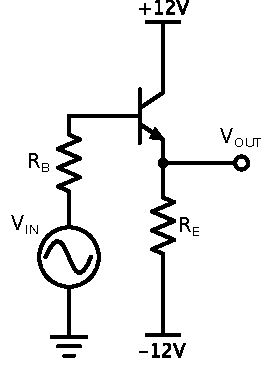
\includegraphics[height=45mm]{cc4.pdf}
	\label{fig:cc4}
\end{wrapfigure}

\subsection{emitter follower polarizzato}
Per polarizzare il transistor, come mostrato dal circuito in Fig. \ref{fig:cc4}, è bastato collegare un capo della resistenza $R_E$ al polo negativo del generatore di corrente continua anziché a massa.

\begin{wrapfigure}[6]{r}[0pt]{36mm}
	\caption{cc5}
	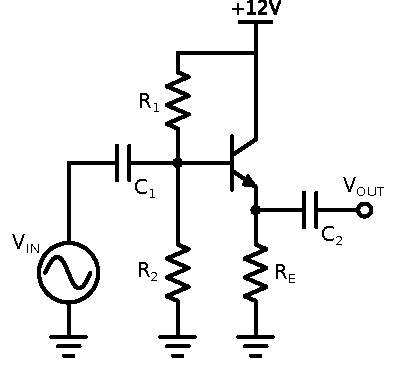
\includegraphics[height=45mm]{cc5.pdf}
	\label{fig:cc5}
\end{wrapfigure}

\subsection{emitter follower con partitore}
Anche in questo caso, poiché avevamo necessità di aggiungere diversi componenti al circuito, abbiamo staccato tutti i componenti dalla breadboard e assemblato il circuito da zero.
